% Proposal (3.5p)
\section{Proposed Method}
\label{sec:proposal}

% General discussion
An autonomous deployment platform should maximize the opportunity to make goals achievable by preparing the system for a broad range of context variability space.


This section describes our method to tackle the challenges presented in~(\ref{sec:challenges}). It consists in offline activities for development of artifacts keeping trace to user goals. And in online support to autonomous handle deployment.

As offline activities, components are defined from a CGM using appropriate patterns. These components are packaged in artifacts together with metadata that describe what goals the packaged component can achieve, its context restrictions and dependencies.

At runtime the adaptation platform receive what goals the user wants to achieve in that environment and look for artifacts that allows it achieve its goals. The platform them assemble and architecture that allows the goal achievement.

\begin{figure*}[!htb]
  \centering
  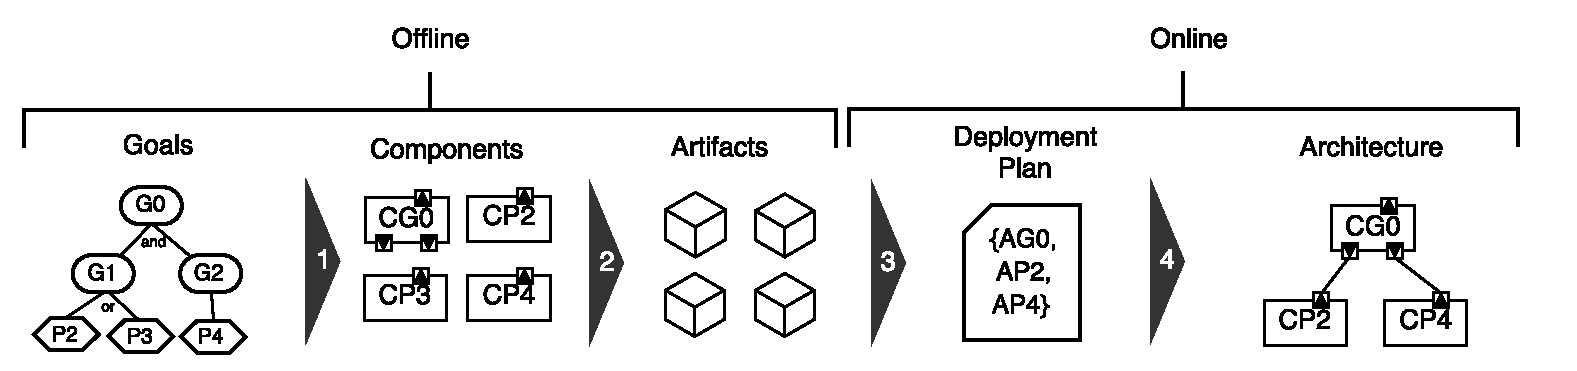
\includegraphics[width=0.8\linewidth]{transformations}
  \caption{Transformations: (1) components definition; (2) packaging; (3) deployment}
\label{fig:overview}
\end{figure*}


Relate Architecture with Requirements.

\begin{figure}[!htb]
  \centering
  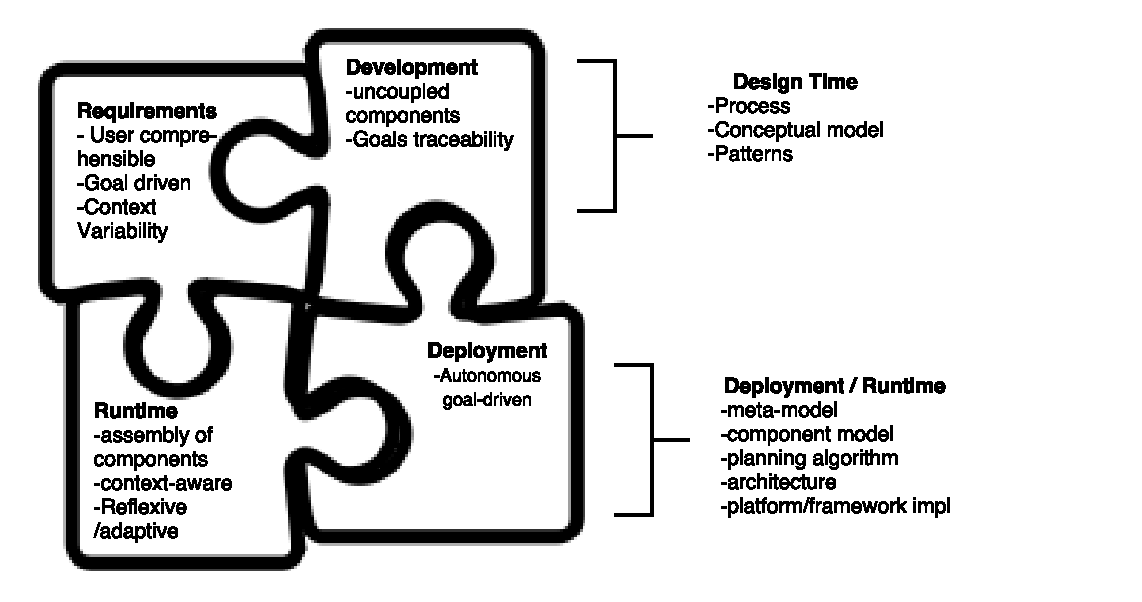
\includegraphics[width=\linewidth]{jig-saw}
  \caption{Proposal Overview}
\label{fig:overview}
\end{figure}



\subsection{Concepts}

\subsubsection{Context and Context Conditions}
\label{context}

In this work we are interested in conditions related with the computing environment. These conditions are related with availability of computing resources, e.g. take a game that can be rendered using CPU or GPU, the availability of GPU is a contextual condition that restrict the achievement of goal render game using GPU strategy.
Adopting the context model proposed in \cite{ali_goal-based_2010} we will express such conditions as formulae in a set of facts. A given context satisfy a context condition if all related facts are monitored and the formulae associated are true.

The facts can be of an atomic proposition such as GPU, that is evaluated to true if an associated resource are known to be available, and it is evaluated to false otherwise.
The facts can be also logical conditions using logical operators ==, !=, <, <=, >, >=.


\subsubsection{Goals, Components and Artifacts}
\label{sec:rules}

We enhance enhance component description with context condition. We extend Yu et al.\cite{yu_goals_2008} patterns for the Goals-Component view with contextual conditions.

\begin{table}[]
\centering
\caption{Contextual Goal Model to components; (1) context condition, (2) And-decomposition, (3)OR-decomposition}
\label{table_related_works}
\begin{tabular}{|l|l|}
\hline
 %\textbf{ A } & \textbf{ B} & \textbf{C} \\ \hline
 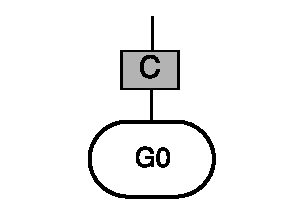
\includegraphics[scale=0.5]{patterns_condition} &
 \begin{lstlisting}
 Component G0 {
   provides IG0;
   condition C;
 }
 \end{lstlisting} \\ \hline
 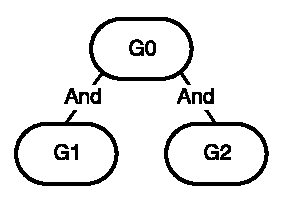
\includegraphics[scale=0.5]{patterns_and_decomposition} &
 \begin{lstlisting}
 Component G0 {
   provides IG0;
   requires IG1, IG2;
 }
 \end{lstlisting} \\ \hline
 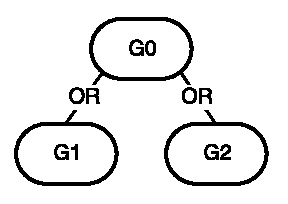
\includegraphics[scale=0.5]{patterns_or_decomposition} &
 \begin{lstlisting}
 Component G1 {
   provides IG0;
 }
 Component G2 {
   provides IG0;
 }
 \end{lstlisting} \\ \hline
\end{tabular}
\end{table}

Software component should be packaged in a standard packaging schema.
The package should, also, have meta-data describing goals it provides, context conditions, and dependencies.

Artifact is a tupla (component, metadata) and metadata is a tupla (context conditions, dependencies, provided goals) context, goals and dependencies.

\begin{itemize}
  \item Context conditions can be evaluated against the context. If the conditions are not satisfied the machine should not deploy the component.
  \item Dependencies are required services that should be provided by other components. Before deploy the component the machine should verify if it can satisfy the dependencies of the component.
  \item Provided goals are services that the component provide to the user or to other components.
\end{itemize}

The artifact dependency: all that its components depend
The artifact provide:  all that its components provide
The artifact conditions:  all that its components conditions

If both context conditions and dependencies are satisfied, the artifact is capable of allow the goal achievement.

\subsubsection{Online Goals}

In traditional goal modeling the agent have a root goal that are refined in subgoals.  Or-refinements allow for variability points in the goal model, but that refinement are static, at least for a given version of the goal model.
We argue that in a dynamic and open environment that vision is not sufficient. We propose a different vision for the autonomous deployment. An agent should have a set of goals that it should pursue. That set can be updated by and user or the agent itself when following a self-assembly approach~\cite{sykes_flashmob:_2011}. We call \emph{active goal} a goal that the agent must pursue.
In a dynamic environment, the agent can at a given moment have or not the resources to achieve a goal. \emph{Achievable Goal} is a goal that the agent pursue and is capable of achieve.

In our deployment view of the goals, we will consider a goal achievable if we can deploy at least one artifact that provide that goals.

\subsubsection{Evolution}

evolve without great effort.

We argue that a goal model can be seen as a protocol definition. When we create OR-Refinements we are giving alternatives of execution, creating variability points.

By creating interfaces in variability points
Open deployment platform.

  and we create opportunity for thirty-parties provide new alternativies

having different context condition will allow the goal to be achievable in a broader range of contexts: for example, in screen controls will allow the game to be playable at touch screen devices.

In tradition deployment schema, a complete new version of the software should be released.

\begin{figure}[!htb]
  \centering
  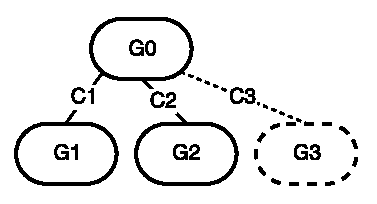
\includegraphics[width=\linewidth]{evolution_or}
  \caption{Evolution OR}
\label{fig:evolution_or}
\end{figure}

Component development and release

\subsubsection{Meta-model}

%TODO Research about goal driven adaptation terminonogy: nelly bencomo

\begin{figure}
  \centering
  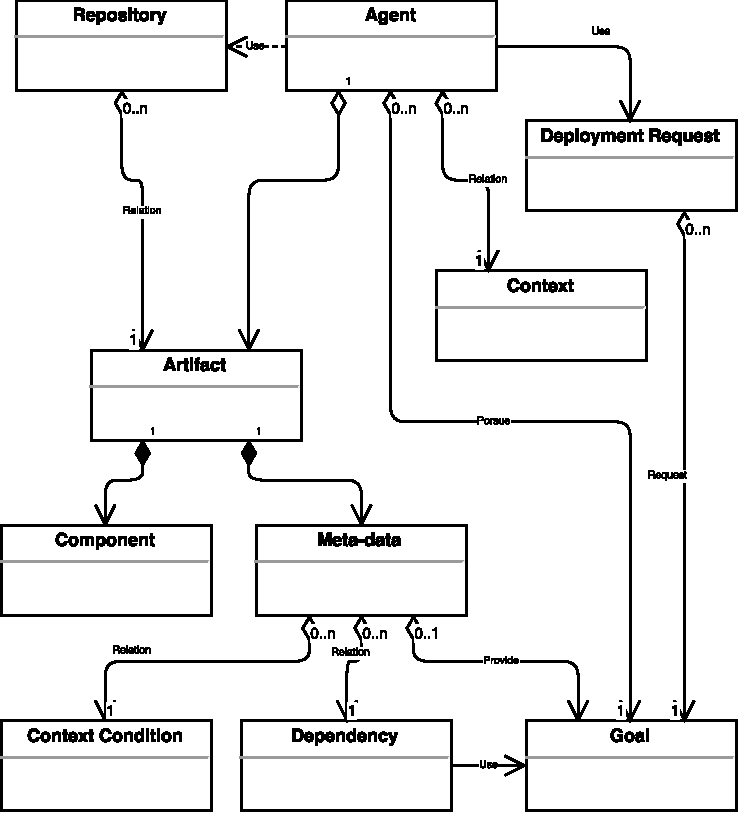
\includegraphics[width=0.8\linewidth]{meta-model}
  \caption{The Goalp Deployment meta-model}
  \label{fig:meta-model}
\end{figure}


\subsection{Off-line}
\label{sec:offline}
%
% The proposed approach is divides in two parts: first, we define a systematic way for a designer specify deployment restrictions to the goal model of the system. Each plan is associated with required computing environment context. We present a Tropos metamodel extension for specify computing environment resources and plans computing environment dependencies.
%
% Second, we introduce an approach for execute the deployment for a given computing environment. The deployment process here encompass deciding with computing resources will be responsible for executing each plan (respecting dependencies restrictions), and which operation needs to be executed in order to realize the deploymet.

%The complete deployment process is illustrated in figure \ref{fig:deployment_process_flow}.

\subsubsection{Roles}
The proposed process considers three roles: users, requirements engineers and software architects.
 Figure~\ref{fig:process_roles} summarize the collaboration between the roles.

\begin{description}
  \item[User]
  This role has access to a particular computing environment and want to achieve some goals there.
  \item[Requirements Engineer]
  Is responsible to translate users goals to a contextual goal model. Also is responsible to analyze the different contexts that the system is meant to operate and how it affects the goals.
  \item[Architect] Architect project the software architecture such as to permit variability of deployment.
  From the point of view of dynamic heterogeneous computing environments, the focus is to create interfaces for components that can allow for goal achievements using different computing resources.

\end{description}

\begin{figure}[!htb]
  \centering
  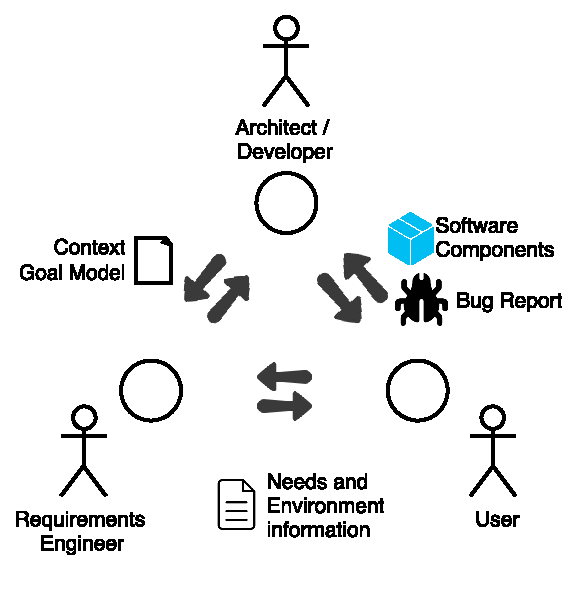
\includegraphics[width=.6\linewidth]{process_roles}
  \caption{Roles collaboration}
\label{fig:process_roles}
\end{figure}

\subsubsection{Activities}

Figure~\ref{fig:deployment_process_flow} describe the development process activities.

\label{sub:Proposal}
\begin{figure}[!htb]
  \centering
  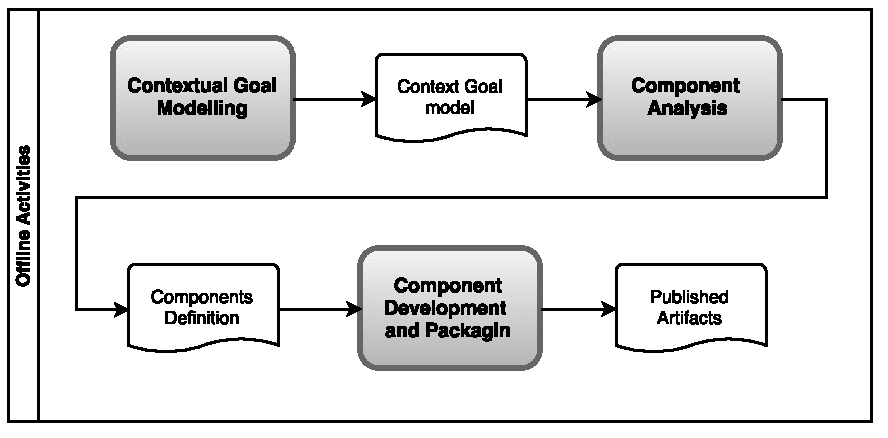
\includegraphics[width=\linewidth]{deployment_process_flow}
  \caption{Deployment Process Activities}
\label{fig:deployment_process_flow}
\end{figure}

\subsubsection{Goal Modeling}
This phase is coordinated by a requirement engineer with participation of a domain specialist, possibly the user.
A process such as TROPOS can be used. The output of this phase is a goal model.
Here, the goal model assumes a central role in the software development process. The goal model besides define the space of the solution, also works as common language. The goal model formalize the domain knowledge. It defines a common language between user and developers that will allow software deployment driven by user goals.


\subsubsection{Context Goal Modeling}
In this phase, the Goal model should be annotated with \emph{context conditions} related with the computing environment. That analysis is a context analysis and could benefit of the process described in~\cite{ali_goal-based_2010}. The requirements engineer should use knowledge about the computing resources that may be available at the computing environment.


\subsubsection{Component Analysis}
Software engineer should identify variability points.
Variability points in the contextual goal model are points where goals can be achieve with different strategies, each one having different context conditions.
Component interfaces are created following the guidelines described in Section~\ref{sec:rules}. The input and output of components are defined.

Also at this phase, it should be defined the sensors needed to evaluate facts about the computing environment.

\subsubsection{Component Development and Packaging}

Component development includes the cycle coding, build and test of software components.
The component package in the standard packaging schema is an artifact and should be put in a delivery system.


\subsubsection{Deployment Actors}

Repository


Node

Artifacts
Interfaces for RC4 open adaptation
Artifacts annotated with requirements and dependencies.


% TODO Relate the challenges with Deployment Manager features


Figure Respository-Platform-Request


\subsection{On-line}
\label{sec:online}


\subsubsection{Deployment Description}

Simple as possible to tackle RC5 (deployment specification accessible to users)


Goal
Subgoals

Mandatory Goals
Optional Goals


Example:
Bomberman

PlayBomberman
Mandatory:BombermanModel
BombermanVideo
BombermanControl
Optional:BombermanAudio

Repo:BombermanControlKeyboard, BombermanControlJoystick


\subsubsection{Goald}
\label{sec:goald}


\begin{figure}[!htb]
  \centering
  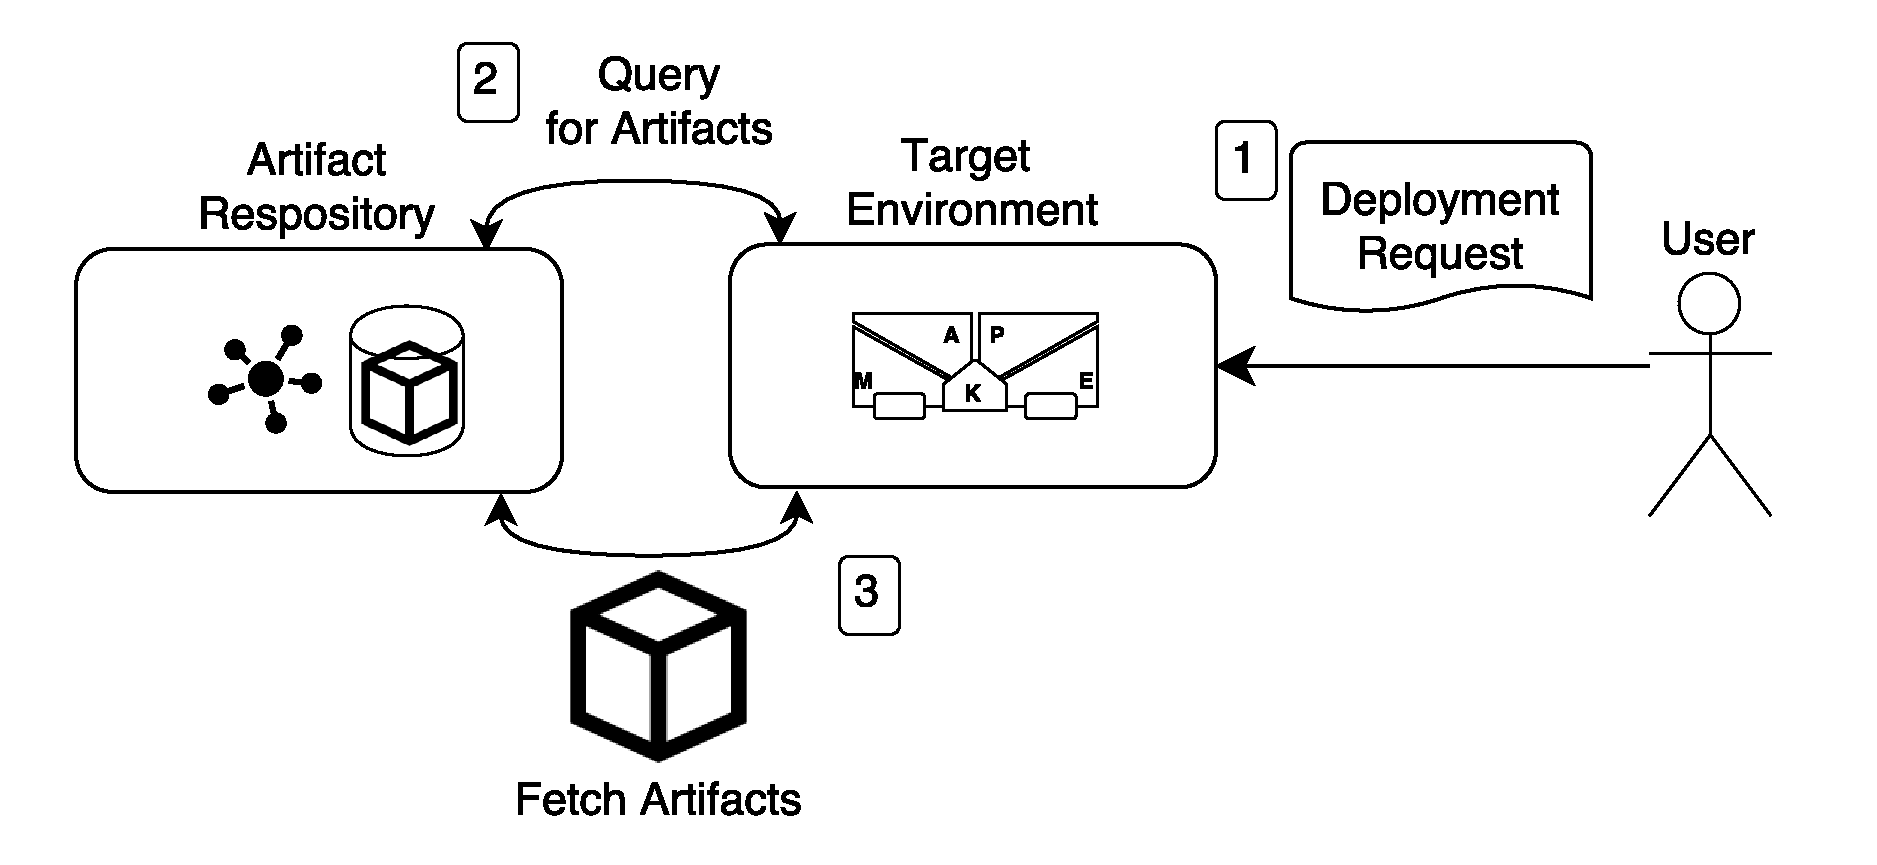
\includegraphics[width=\linewidth]{deployment_actors}
  \caption{Goald Deployment Actors}
\label{fig:deployment_actors}
\end{figure}

Figure~\ref{fig:deployment_actors} depicts the deployment execution. A user interested in using a computing environment to achieve a set of goals submits to this environment which goals it want to achieve in the form of a deployment request.

Then, our system introspect about available computing resources and artifacts present in repository and plan the deployment, generating a deployment plan that is a selection of artifacts that can allow for the goals achievement in the available computing environment. The deployment is them executed by fetching the appropriate artifacts from the repositories.

Facts about the computing environment are directed monitored by the agent by means of sensors. An Artifact should have in its meta-data the condition for its deployment. That condition is specified by a formula of facts.

\subsubsection{Deployment Manager}

Deployment Operations
install
uninstall

\subsubsection{Component Model}
\begin{itemize}
  \item Requirements
  \item Dependencies
\end{itemize}

\begin{itemize}
    \item Information it queries
    \item Listened Events
    \item Dispatched Events
    \item Periodic Execution
\end{itemize}


Life cycle

\begin{figure}[!htb]
  \centering
  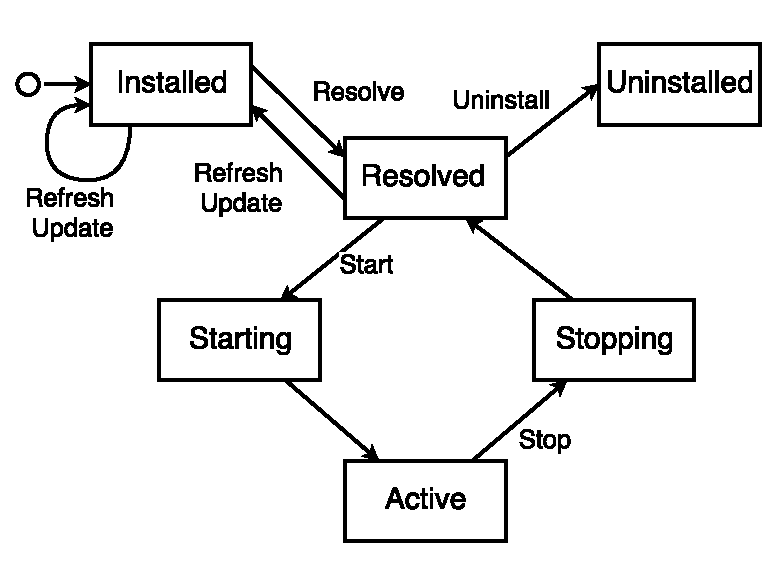
\includegraphics[width=.6\linewidth]{component_life_cycle}
  \caption{Component Life Cycle}
\label{fig:component_life_cycle}
\end{figure}


\begin{itemize}
  \item install
  \item register (listeners)
  \item uninstall
\end{itemize}

Dynamic binding

\subsubsection{Application}

Escalonando a aplicação e o código de adaptação.

\subsubsection{Initial Setup}

Knowledge base,
Component model of the platform: mape-k is in it self a component.



\subsubsection{Illustrative Scenarios}
New Goal

Adapt to resource failure


\subsubsection{Open Adaptation}

\subsubsection{Evolution 1: Notify user about not achievable goals}
If a goal is not achievable a event is generated. With this another component can take action such as notify a external agent (e.g a user) that a goal is not achievable locally with current resources and known components.


\subsubsection{Evolution 2: Adaptive monitoring policies}
% Monitoring policy
A monitor is associated with a monitoring policy that dictate the periodicy that the sense should occur.
\begin{itemize}
  \item periódico:
  \item on demand: Is executed in response to a query
  \item listener: Is called by another system component or external actor.
\end{itemize}



\subsubsection{Addressing Challenges}
RC1 uncertainty at design time and RC2 heterogeneous computing environment

We address these challenges by assembling the system at runtime driven by user goals. Using our approach the developer do not need to know the exact specification of the user environment.
We tackle challenge RC2 (heterogeneous computing environment) using decentralized approach to handle variability of computing environment.

RC3 dynamism
We address this challenge by providing an adaptation framework to handle changes in the computing environment.
Analyzing and responding to changes in the computing environment.

RC4 open adaptation
We address this challenge by providing descentralized approach based on interfaces so that third party developers can provide new components to the system at runtime.


RC5 deployment specification accessible to users
We address this by using goals as abstract way of specifying the system deployment. By this the user do not need to know details about system administration to configure a system. In our approach system administration rules and policies can be implemented as components.


\subsubsection{Architecture}

\begin{figure}[!htb]
  \centering
  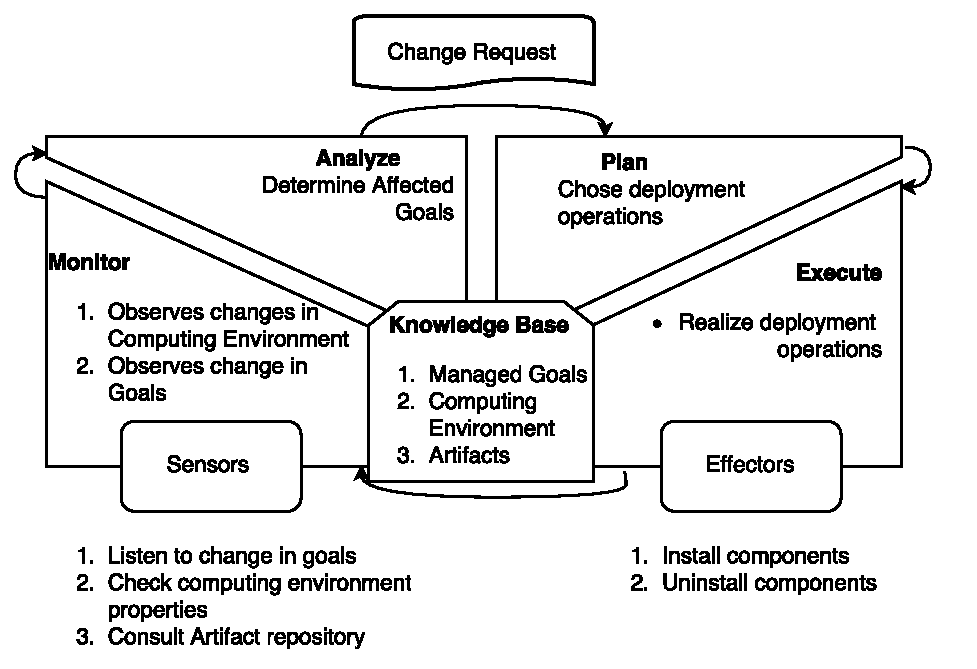
\includegraphics[width=\linewidth]{goald_mape_k}
  \caption{Goald Deployment Manager}
\label{fig:goald_mape_k}
\end{figure}

\begin{itemize}
  \item events: are handled to registered listeners.
\end{itemize}

\subsubsection{Knowledge Base}

The knowledge base store a model of goals the system much achieve, the computing environment context and current deployed artifacts.

The information in the knowledge base can be of two types:
\begin{itemize}
  \item facts: can be queried about by registered components
\end{itemize}


\subsubsection{Monitors}

Monitors are components that observes changes in the goals and context. All
\begin{itemize}
  \item Goal Change Monitor is responsible for listening to request of include or remove goals.
  \item Computing Environment monitor is responsible to verify \emph{facts} about the computing enivronment as introduced in~\ref{context}. \emph{Facts} are stored in the Knowledge Base and used to evaluate context conditions.
  \item Repository monitors observe changes in software repositories.
  \item Introspective monitors observe the system state and behavior. (ex: monitor that check if there is any monitor that dispatches events that no one cares about)
\end{itemize}

The result of monitors can be:
\begin{itemize}
  \item Change the knowledge base
  \item Dispatch Events
\end{itemize}

Core Components:
\begin{itemize}
  \item Timer Monitoring Policy:
  \item Computing Environment Sensors: listen to timeouts of monitoring policy. Sense the environment. Update the knowledge base and dispatch events for changes in the environment.
  \item Goals change listeners: listen for external entities that want to change the goals of the machine. The interface is implementation dependent (e.g HTTP service, GUI, command line). Dispatch External Change Requests.
  \item Repository Monitor: queries repository for information about components.
\end{itemize}



\subsubsection{Analyzer}

Objective change analyzer

Computing environment change - evaluate if any system goal is affected.

Evaluate parametric formula for managed goals. If a goal probability of success drops below a threshold, dispatch deployment replanting event.

Handling evolution: simple approach favor a superior version.


\begin{itemize}
  \item Goals Change- Check if a goal request is a change request. A goal removal will affect another goals?

  \item Adaptation
In case of change in the available resources
it should be analyzed if the change threats the achievements of goals.

\end{itemize}

Listens to:
\begin{itemize}
  \item changes in the environment
  \item external changes in goals
\end{itemize}

Dispatch
\begin{itemize}
  \item Change Request: request a change in the deployment. Contains affected goals for what deployment should be replanned.
\end{itemize}

\subsubsection{Planner}

Receive change requests and enqueue it.

Deployment Change Planner is responsible for finding which operation should be executed in order to (1) make the active goals achievable. (2) Free up resource not associated with active goals.

How deployment is planned and the algorithm used will be described in Section~\ref{sec:deployment_planning}.

Components
\begin{itemize}
  \item Context Evaluation: it is responsible to evaluate if context conditions are satisfied for a given component in a given context.
\end{itemize}

Listens To:
\begin{itemize}
  \item Change Request
\end{itemize}

Dispatch:
\begin{itemize}
  \item Query Repositories: request information about available components that provide given goals.
  \item Execute Plan: request a deployment plan to be executed.
\end{itemize}



\subsubsection{Execute}

Executor components are responsible to actuate in the system.
Deployment Change Executor is responsible for get components from repository and execute deployment operations such as install and uninstall components.

% Fix Resource

% Change monitoring policy

Listen To:
\begin{itemize}
  \item Execute Plan:
\end{itemize}


\section{Deployment Planning}
\label{sec:deployment_planning}

Planning for new goals.

A goal is deployable if all its context conditions and dependencies are satisfiable. If a goal is satisfiable there is a deployment plan that is able to satisfy this goal. A deployment plan consist of a set of artifacts that form a closure in the dependency graph and all nodes has context conditions satisfiable.

\begin{figure}[!htb]
  \centering
  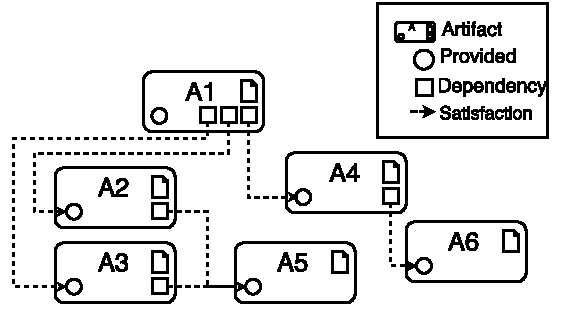
\includegraphics[width=.6\linewidth]{dependency_graph}
  \caption{Dependency Graph}
  \label{fig:dependency_graph}
\end{figure}

\begin{algorithm}
 \KwIn{A goal}
 \KwResult{DeploymentPlan plan}
 \caption{doPlanDeployment(Goal goal)}
 \label{alg:deployment_plan}

 List [] artifacts $\leftarrow$ getArtifactsThatProvide(goal)\;
 \ForEach{Artifact artifact in artifacts}{
   	Boolean contextSatisfaction $\leftarrow$ isSatisfied(artifact.contextConditions)\;
    \If{contextSatisfaction}{
      DeploymentPlan plan $\leftarrow$ new DeploymentPlan()\;
      \ForEach{Goal dependency in artifact.dependencies}{
          DeploymentPlan subPlan  $\leftarrow$ doPlanDeployment(dependency)\;
          \If{!dependencySatisfaction == NULL}{
            \Return{NULL}
          }\Else{
            plan.add(subPlan);
          }
      }
      \Return{plan}
    }\Else{
      \Return{NULL}
    }
  }
\end{algorithm}

